\documentclass[]{article}
\usepackage[a4paper, total={15cm,23cm}]{geometry}
\usepackage{fancyhdr}
\usepackage{graphicx}
\usepackage{amsmath}
\usepackage{amssymb}
\usepackage[dvipsnames]{xcolor}
\usepackage{tikz}
\usepackage{verbatim}
\usepackage{tcolorbox}
\usepackage{textcomp}
\usepackage{xcomment}
\usepackage{xstring}
%opening
\title{Magnetic Field of a Partially Curved Wire}
\author{Benjamin Bauml and Danielle Skinner}
\date{Winter 2024}
\pagestyle{fancy}
\rhead{PH 223}
\chead{Winter 2024}
\lhead{Week 10}

% Version 2024-02-21
% Changes
% 2024-02-21 Added xstring package to enable smooth implementation of new \ModePage command.
% For Assignment, leave Purpose as 1. For Worksheet, set to 2. For Student Solution, set to 3. For Teacher Solution, set to 4.
\newcommand{\Purpose}{4}

\newcommand{\Exclusion}{0}
\newcommand{\PageTurn}{0}
\newcommand{\GrayProb}{0}
\newcommand{\Tipsy}{0}

% Assignment
\if\Purpose1
\renewcommand{\Exclusion}{1}
\fi
% Worksheet
\if\Purpose2
\renewcommand{\Exclusion}{1}
\renewcommand{\PageTurn}{1}
\fi
% Student Solution
\if\Purpose3
\renewcommand{\PageTurn}{1}
\renewcommand{\GrayProb}{1}
\fi
% Teaching Copy
\if\Purpose4
\renewcommand{\PageTurn}{1}
\renewcommand{\GrayProb}{1}
\renewcommand{\Tipsy}{1}
\fi

\if\Exclusion1
\xcomment{Title,Problem,ProblemSub,PassFig}
\fi

\def \NewQ {0}
\def \PForce {0}
\newcommand{\MaybePage}[1]{
	\def \PForce {#1}
	\if\PForce1
		\newpage
	\else
		\if\NewQ0
		\gdef \NewQ {\PageTurn}
		\else
		\newpage
		\fi
	\fi
}

\newcommand{\ModePage}[1]{
	\IfSubStr{#1}{\Purpose}{\newpage}{}
}

\newenvironment{Problem}[2][0]{%The first argument is optional, and if it is set to 1, the \newpage will be forced.
\MaybePage{#1}
\section*{#2}
\if\GrayProb1
\begin{tcolorbox}[colback=lightgray,colframe=lightgray,sharp corners,boxsep=1pt,left=0pt,right=0pt,top=0pt,bottom=0pt,after skip=2pt]
\else
\begin{tcolorbox}[colback=white,colframe=white,sharp corners,boxsep=1pt,left=0pt,right=0pt,top=0pt,bottom=0pt,after skip=2pt]
\fi
}{
\end{tcolorbox}\noindent
}

\newenvironment{ProblemSub}[1][0]{%The argument is optional, and if a string of numbers is entered into it, it will force a \newpage in any \Purpose that shows up in the string. For example, "13" would lead to the newpage being forced in modes 1 and 3.
\ModePage{#1}
\if\GrayProb1
\begin{tcolorbox}[colback=lightgray,colframe=lightgray,sharp corners,boxsep=1pt,left=0pt,right=0pt,top=0pt,bottom=0pt,after skip=2pt]
\else
\begin{tcolorbox}[colback=white,colframe=white,sharp corners,boxsep=1pt,left=0pt,right=0pt,top=0pt,bottom=0pt,after skip=2pt]
\fi
}{
\end{tcolorbox}\noindent
}

\newenvironment{PassFig}{\begin{figure}[h]}{\end{figure}}

\newcommand{\TeachingTips}[1]{
\if\Tipsy1
\begin{tcolorbox}[colback=lightgray,colframe=black]
#1
\end{tcolorbox}
\fi
}

\newenvironment{Title}{\maketitle}{}

\begin{document}
\begin{Title}
\begin{center}
	This problem is from the Week 9 Help and Practice Problems for PH 213, and probably was originally sourced from \textit{Physics for Scientists and Engineers}.
\end{center}
\end{Title}

\begin{Problem}{Activity 1}
	Use the Biot-Savart law to find the magnetic field strength at the center of the semicircle in the figure below.
\end{Problem}
\begin{PassFig}
	\centering
	%\includegraphics[scale=0.5]{curved_wire.png}
	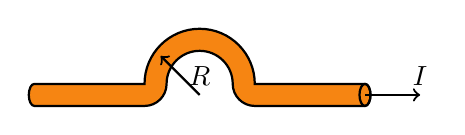
\begin{tikzpicture}[scale=0.7]
		\filldraw[thick,color=black,fill=BurntOrange] (-1,0.2) arc (180:0:1) -- (3,0.2) arc (90:-90:0.1 and 0.2) -- (1,-0.2) arc (270:180:0.4) arc (0:180:0.6) arc (0:-90:0.4) -- (-3,-0.2) arc (270:90:0.1 and 0.2) -- cycle;
		\draw[thick] (3,0) ellipse (0.1cm and 0.2cm);
		\draw[thick,->] (0,0) -- ({cos(135)},{sin(135)});
		\node[anchor=south] at (0,0) {$R$};
		\draw[thick,->] (3,0) -- (4,0);
		\node[anchor=south] at (4,0) {$I$};
	\end{tikzpicture}
\end{PassFig}

We will tackle this problem using the Chop-Multiply-Add method.
The Biot-Savart law is:
\[
	\vec{B} = \frac{\mu_o}{4\pi}\frac{q\vec{v}\times\hat{r}}{r^2}	
\]

Let's first consider the magnetic field due to the two straight sides. The current moves in the $+\hat{x}$ direction, and the $\hat{r}$ is in the $\pm\hat{x}$. Therefore the cross-product in the Biot-Savart law is zero. The straight sides don't contribute a magnetic field to the center of the loop. So we only need to focus on the curved portion!

\begin{figure}[h]
	\centering
	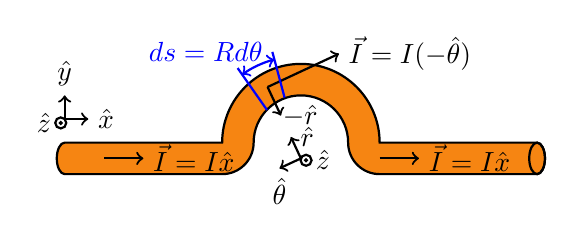
\begin{tikzpicture}
		\filldraw[thick,color=black,fill=BurntOrange] (-1,0.2) arc (180:0:1) -- (3,0.2) arc (90:-90:0.1 and 0.2) -- (1,-0.2) arc (270:180:0.4) arc (0:180:0.6) arc (0:-90:0.4) -- (-3,-0.2) arc (270:90:0.1 and 0.2) -- cycle;
		\draw[thick] (3,0) ellipse (0.1cm and 0.2cm);
		\draw[thick,->] (0,0) -- ({0.3*cos(115)},{0.3*sin(115)});
		\node[anchor=west] at ({0.3*cos(115)},{0.3*sin(115)}) {$\hat{r}$};
		\draw[thick,->] (0,0) -- ({-0.3*sin(115)},{0.3*cos(115)});
		\node[anchor=north] at ({-0.3*sin(115)},{0.3*cos(115)}) {$\hat{\theta}$};
		\filldraw ({-0.07*cos(160)},{-0.07*sin(160)}) circle (0.02);
		\draw[thick] ({-0.07*cos(160)},{-0.07*sin(160)}) circle (0.07);
		\node[anchor=west] at ({-0.07*cos(160)},{-0.07*sin(160)}) {$\hat{z}$};
		\draw[thick,->] ({cos(115)},{sin(115)}) -- ({cos(115)+1*sin(115)},{sin(115)-1*cos(115)});
		\node[anchor=west] at ({cos(115)+1*sin(115)},{sin(115)-1*cos(115)}) {$\vec{I} = I(-\hat{\theta})$};
		\draw[thick,->] ({cos(115)},{sin(115)}) -- ({cos(115)-0.4*cos(115)},{sin(115)-0.4*sin(115)});
		\node[anchor=west] at ({cos(115)-0.4*cos(115)-0.1},{sin(115)-0.4*sin(115)}) {$-\hat{r}$};
		\begin{scope}[rotate=-55]
			\draw[thick,blue] (-0.75,0) -- (-1.4,0);
		\end{scope}
		\begin{scope}[rotate=-75]
			\draw[thick,blue] (-0.8,0) -- (-1.4,0);
		\end{scope}
		\begin{scope}[rotate=-55]
			\draw[thick,blue,<->] (-1.3,0) arc (180:160:1.3);
		\end{scope}
		\node[anchor=east] at ({-1.4*cos(75)},{1.4*sin(75)}) {\color{blue}$ds = Rd\theta$};
		\begin{scope}[shift={(-2.5,0)}]
			\draw[thick,->] (0,0) -- (0.5,0);
			\node[anchor=west] at (0.5,0) {$\vec{I}=I\hat{x}$};
		\end{scope}
		\begin{scope}[shift={(1,0)}]
			\draw[thick,->] (0,0) -- (0.5,0);
			\node[anchor=west] at (0.5,0) {$\vec{I}=I\hat{x}$};
		\end{scope}
		\begin{scope}[shift={(-3,0.5)}]
			\draw[thick,->] (0,0) -- (0.3,0);
			\node[anchor=west] at (0.3,0) {$\hat{x}$};
			\draw[thick,->] (0,0) -- (0,0.3);
			\node[anchor=south] at (0,0.3) {$\hat{y}$};
			\filldraw ({-0.07*cos(45)},{-0.07*sin(45)}) circle (0.02);
			\draw[thick] ({-0.07*cos(45)},{-0.07*sin(45)}) circle (0.07);
			\node[anchor=east] at ({-0.07*cos(45)},{-0.07*sin(45)}) {$\hat{z}$};
		\end{scope}
	\end{tikzpicture}
\end{figure}

Starting with the ``Chop" part, we can rewrite the cross product:
\[
	dq\vec{v}\times\hat{r} = ds\vec{I}\times\hat{r} = (Rd\theta)I(-\hat{\theta}) \times (-\hat{r}) = IRd\theta (-\hat{z}).
\]
To do this calculation, we switched to a cylindrical coordinate system. The current moves in the $-\hat{\theta}$ direction, and the $\hat{r}$ points from the wire to the center of the semi-circle, making it negative.

\TeachingTips{
\[
dq\cdot v = dq\cdot\frac{ds}{dt} = ds\cdot\frac{dq}{dt} = ds\cdot I 
\]
}

Now on to ``Multiply.'' The infinitesimal magnetic field can now be written as
\[
	d\vec{B} = \frac{\mu_o}{4\pi}\frac{dq\vec{v}\times\hat{r}}{r^2} = \frac{\mu_o}{4\pi}\frac{IRd\theta}{R^2} (-\hat{z}).
\]
Finally, the ``Add'':
\[
	\vec{B} = \frac{\mu_o}{4\pi}\frac{I}{R}(-\hat{z})\int_{0}^{\pi} d\theta.
\]
The final answer is therefore
\[
	\vec{B} = \frac{\mu_o}{4}\frac{I}{R}(-\hat{z}).
\]
We can see that this is half the result of a magnetic field due to a current loop!
\end{document}
